\documentclass[tikz,border=10pt]{standalone}
\begin{document}
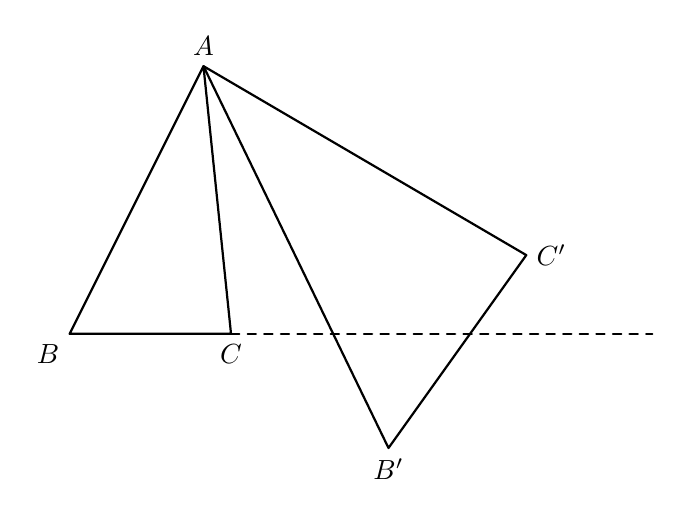
\begin{tikzpicture}[line cap=round,line join=round,thick]

\coordinate (A) at (0,3.4);
\coordinate (B) at (-1.7,0);
\coordinate (C) at (0.35,0);
\coordinate (Bp) at (2.35,-1.45);
\coordinate (Cp) at (4.1,1.0);

\draw (A) -- (B) -- (C) -- cycle;
\draw (A) -- (Bp) -- (Cp) -- cycle;
\draw[dashed] (C) -- (5.7,0);

\node[above] at (A) {$A$};
\node[below left] at (B) {$B$};
\node[below] at (C) {$C$};
\node[below] at (Bp) {$B'$};
\node[right] at (Cp) {$C'$};

\end{tikzpicture}
\end{document}
